%----------------------------------------------------------------------------------------
%	SOLUTION 1.a
%----------------------------------------------------------------------------------------
\subsection*{Problem 1.a}
It is given that
\begin{align*}
	\hat{y} = \sin\phi.
\end{align*}
If $\phi \sim U[0,\pi]$ then pdf of $\phi$ is given by
\begin{align*}
	f_{\Phi}(\phi) &= \frac{1}{\pi}.
\end{align*}
Now, when $\phi \in [0,\frac{\pi}{2}]$,
\begin{align*}
	f_{\hat{Y}}(\hat{y}) &= \frac{f_{\Phi}(\phi)}{|\frac{\partial \hat{y}}{\partial \phi}|}\\
	&= \frac{\frac{1}{\pi}}{\cos \phi}.
\end{align*}
Therefore, $\cos \phi = \frac{1}{\pi f_{\hat{Y}}(\hat{y})}$. Hence,
\begin{align*}
	&\cos^2 \phi + \sin^2 \phi = 1\\
	\implies & \frac{1}{\pi^2 f_{\hat{Y}^2(\hat{y})}} + \hat{y}^2 = 1\\
	\implies & \frac{1}{f_{\hat{Y}(\hat{y})}} = \pi\sqrt{1-\hat{y}^2}\\
	\implies & f_{\hat{Y}(\hat{y})} = \frac{1}{\pi\sqrt{1-\hat{y}^2}}
\end{align*}
We can find a similar solution when  $\phi \in [\frac{\pi}{2}, \pi]$,
Therefore,
\begin{align*}
	f_{\hat{Y}}(\hat{y}) = \begin{cases}
		\frac{2}{\pi\sqrt{1-\hat{y}^2}},\ \text{ if }y\in[0,1]\\
		0,\ \text{ otherwise }.
	\end{cases}
\end{align*}
%----------------------------------------------------------------------------------------
%	SOLUTION 1.b
%----------------------------------------------------------------------------------------
\subsection*{Problem 1.b}
\begin{align*}
	E[\hat{Y}] &= \int_{-\infty}^{\infty} \hat{y}f_{\hat{Y}}(\hat{y})\text{d}\hat{y}\\
	&= \int_{0}^{1}\frac{2\hat{y}}{\pi\sqrt{1-\hat{y}^2}}\text{d}\hat{y}.
\end{align*}
Let $k^2 = 1-\hat{y}^2$. Then, $\hat{y}\text{d}\hat{y} = -k\text{d}k$.
So,
\begin{align*}
	E[\hat{Y}] &= \frac{2}{\pi}\int_{0}^{1}\text{d}k\\
	&= \frac{2}{\pi}\\
	&= 0.6366.
\end{align*}
Now,
\begin{align*}
	E[\hat{Y}^2] &= \int_{-\infty}^{\infty} \hat{y}^2f_{\hat{Y}}(\hat{y})\text{d}\hat{y}\\
	&= \frac{2}{\pi}\int_{0}^{1}\frac{\hat{y}^2}{\sqrt{1-\hat{y}^2}}\text{d}\hat{y}.\\
\end{align*}
Let $\hat{y} = \sin k$, then $\text{d}\hat{y} = \cos k \text{d}k$. Therefore,
\begin{align*}
	\int \frac{\hat{y}^2}{\sqrt{1-\hat{y}^2}}\text{d}\hat{y} &= \int \frac{\sin^2 k}{\cos k}\cos k\text{d}k\\
	&= \int \frac{1}{2}(1-\cos (2k))\text{d}k\\
	&= \frac{k}{2}-\frac{1}{4}\int 2 \cos (2k)\text{d}k+C_1\\
	&= \frac{k}{2}-\frac{1}{4}\sin (2k)+C_2\\
	&= \frac{k}{2}-\frac{1}{2}\sin k \cos k + C_2\\
	&= \frac{1}{2}(\sin^{-1}\hat{y})-\frac{1}{2}\hat{y}\sqrt{1-\hat{y}^2}+C_2.
\end{align*}
Considering the limits of the integral, we get,
\begin{align*}
	E[\hat{Y}^2] = \frac{2}{\pi}\frac{1}{2}\left[\frac{\pi}{2}\right] = \frac{1}{2}.
\end{align*}
Therefore,
\begin{align*}
	Var(\hat{Y}) &= E[\hat{Y}^2]-(E[\hat{Y}])^2\\
	&= \frac{1}{2}-\frac{4}{\pi^2}\\
	&= \frac{\pi^2-8}{2\pi^2}\\
	&= 0.0947.
\end{align*}
%----------------------------------------------------------------------------------------
%	SOLUTION 1.c
%----------------------------------------------------------------------------------------
\subsection*{Problem 1.c}
From the Monte Carlo simulation I get the following:
\begin{align*}
	E[\hat{Y}_{mc}] &= 0.635\\
	\text{Var}(\hat{Y}_{mc}) &= 0.096.
\end{align*}
Fig.~\ref{fig:q1_unif_phi_mc} shows the plot of analytically computed PDF of $\hat{Y}$ and PDF histogram of $\hat{Y}$ from Monte Carlo simulation. The figure reveals that both analytical and Monte Carlo results are similar. Also, the mean and variance of $\hat{Y}$ from Monte Carlo are close enough to analytical results.
\begin{figure}[!h]
	\centering
	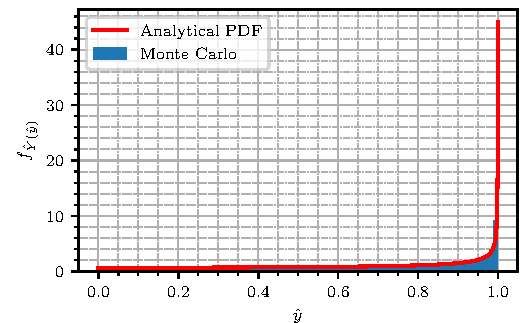
\includegraphics[scale=1.0,trim={0cm 0cm 0cm 0cm},clip]{./code/generatedPlots/q1_unif_phi_mc.pdf}
	\caption{Q1.c: Analytical vs. Monte Carlo PDF of $\hat{Y}$ when $\phi \sim U[0,\pi]$}
	\label{fig:q1_unif_phi_mc}
\end{figure}
%----------------------------------------------------------------------------------------
%	SOLUTION 1.d
%----------------------------------------------------------------------------------------
\subsection*{Problem 1.d}
I have used Monte Carlo simulation for this part. When $\phi \sim \mathcal{N}(0,1)$, from Monte Carlo simulation, I get the following:
\begin{align*}
	E[\hat{Y}_{mc}] &= 0.007\\
	\text{Var}(\hat{Y}_{mc}) &= 0.432.
\end{align*}
The histogram based PDF of $\hat{Y}$ is shown in Fig.~\ref{fig:q1_norm_phi_mc}, when $\phi \sim \mathcal{N}(0,1)$
\begin{figure}[!h]
	\centering
	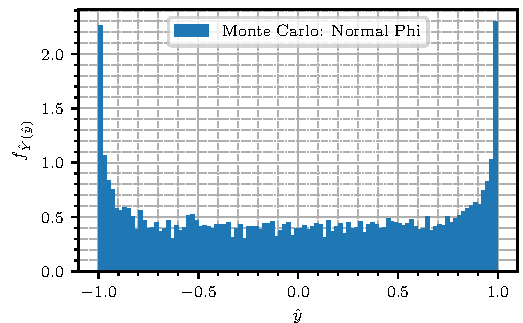
\includegraphics[scale=1.0,trim={0cm 0cm 0cm 0cm},clip]{./code/generatedPlots/q1_norm_phi_mc.pdf}
	\caption{Q1.c:  Monte Carlo PDF of $\hat{Y}$ when $\phi \sim \mathcal{N}(0,1)$}
	\label{fig:q1_norm_phi_mc}
\end{figure}


I used Monte Carlo approach for this problem as calculating the PDF of $\hat{Y}$ under the non-linear transformation when $\phi \sim \mathcal{N}(0,1)$ is much harder and even deducing the mean of variance of it is much harder compared to Monte Carlo simulation. This is an example of how non-linear transformation of random variables result into very difficult analytical expression. 